\documentclass[12pt]{article}

\usepackage{amssymb,amsmath,amsthm}
\usepackage[top=1in, bottom=1in, left=1.25in, right=1.25in]{geometry}
\usepackage{fancyhdr}
\usepackage{enumerate}
\usepackage[bw,framed,numbered]{mcode}
\usepackage{graphicx}

% Comment the following line to use TeX's default font of Computer Modern.
\usepackage{times,txfonts}

\newtheoremstyle{homework}% name of the style to be used
  {18pt}% measure of space to leave above the theorem. E.g.: 3pt
  {12pt}% measure of space to leave below the theorem. E.g.: 3pt
  {}% name of font to use in the body of the theorem
  {}% measure of space to indent
  {\bfseries}% name of head font
  {:}% punctuation between head and body
  {2ex}% space after theorem head; " " = normal interword space
  {}% Manually specify head
\theoremstyle{homework} 

% Set up an Exercise environment and a Solution label.
\newtheorem*{exercisecore}{Exercise \@currentlabel}
\newenvironment{exercise}[1]
{\def\@currentlabel{#1}\exercisecore}
{\endexercisecore}

\newcommand{\localhead}[1]{\par\smallskip\noindent\textbf{#1}\nobreak\\}%
\newcommand\solution{\localhead{Solution:}}

%%%%%%%%%%%%%%%%%%%%%%%%%%%%%%%%%%%%%%%%%%%%%%%%%%%%%%%%%%%%%%%%%%%%%%%%
%
% Stuff for getting the name/document date/title across the header
\makeatletter
\RequirePackage{fancyhdr}
\pagestyle{fancy}
\fancyfoot[C]{\ifnum \value{page} > 1\relax\thepage\fi}
\fancyhead[L]{\ifx\@doclabel\@empty\else\@doclabel\fi}
\fancyhead[C]{\ifx\@docdate\@empty\else\@docdate\fi}
\fancyhead[R]{\ifx\@docauthor\@empty\else\@docauthor\fi}
\headheight 15pt

\def\doclabel#1{\gdef\@doclabel{#1}}
\doclabel{Use {\tt\textbackslash doclabel\{MY LABEL\}}.}
\def\docdate#1{\gdef\@docdate{#1}}
\docdate{Use {\tt\textbackslash docdate\{MY DATE\}}.}
\def\docauthor#1{\gdef\@docauthor{#1}}
\docauthor{Use {\tt\textbackslash docauthor\{MY NAME\}}.}
\makeatother

% Shortcuts for blackboard bold number sets (reals, integers, etc.)
\newcommand{\Reals}{\ensuremath{\mathbb R}}
\newcommand{\Nats}{\ensuremath{\mathbb N}}
\newcommand{\Ints}{\ensuremath{\mathbb Z}}
\newcommand{\Rats}{\ensuremath{\mathbb Q}}
\newcommand{\Cplx}{\ensuremath{\mathbb C}}
%% Some equivalents that some people may prefer.
\let\RR\Reals
\let\NN\Nats
\let\II\Ints
\let\CC\Cplx

%%%%%%%%%%%%%%%%%%%%%%%%%%%%%%%%%%%%%%%%%%%%%%%%%%%%%%%%%%%%%%%%%%%%%%%%%%%%%%%%%%%%%%%
%%%%%%%%%%%%%%%%%%%%%%%%%%%%%%%%%%%%%%%%%%%%%%%%%%%%%%%%%%%%%%%%%%%%%%%%%%%%%%%%%%%%%%%
% 
% The main document start here.

% The following commands set up the material that appears in the header.

%%%%%%%%%%%%%%%%%%%%%%%%%%%%%%%%%%%%%%%%%%%%%%%%%%%%%%%%%%%%%%%%%%%%%%%%%%%%%%%%%%%%%%%
%%%%%%%%%%%%%%%%%%%%%%%%%%%%%%%%%%%%%%%%%%%%%%%%%%%%%%%%%%%%%%%%%%%%%%%%%%%%%%%%%%%%%%%
% 
% The main document start here.

% The following commands set up the material that appears in the header.
\doclabel{Math 310: Homework 2}
\docauthor{Parker Whaley}
\docdate{August 22, 2016}

\newcommand{\vv}{\mathbf{v}}
\begin{document}

\begin{exercise}{1}
Write a small Matlab function largest(a,b) that returns the largest of the two values.
Test that your function works by computing largest(1,2), largest(0,-1) and
largest(5,5).
\end{exercise}

\lstinputlisting{../octave/largest.m}
\lstinputlisting{../octave/largest_log.txt}
\newpage
\begin{exercise}{2}
Write a small Matlab function nextprime(x) that takes a positive integer argument and
returns the smallest prime number at least as large as x. Your function should use a while
loop and take advantage of the isprime function in Matlab. Test that your function
works by computing nextprime(5), nextprime(6), nextprime(-1) and nextprime(100).

\end{exercise}
\lstinputlisting{../octave/nextprime.m}
\lstinputlisting{../octave/nextprime.txt}
\newpage
\begin{exercise}{3}
Define a sequence of numbers by $x_1 = 1$ and $x_{k+1} =\frac{1}{2}x_k + 1$. Write a Matlab function
buildseq(N) that returns an array with the first N elements of the sequence in it. For
example, buildseq(2) should return [1, 1.5]. Test that your function works by computing
the first four sequence elements by hand, and then verifying that your function computes
them correctly. You may wish to take advantage of the Matlab command zeros.
\end{exercise}
\lstinputlisting{../octave/buildseq.m}
\lstinputlisting{../octave/buildseq.txt}

\newpage
\begin{exercise}{Chapter 4: 2(a)}
\end{exercise}
This is my bisect method
\lstinputlisting{../octave/findzero.m}

The script to solve
\lstinputlisting{../octave/question_4.m}

\newpage
And the result of the script
\lstinputlisting{../octave/q4a.txt}
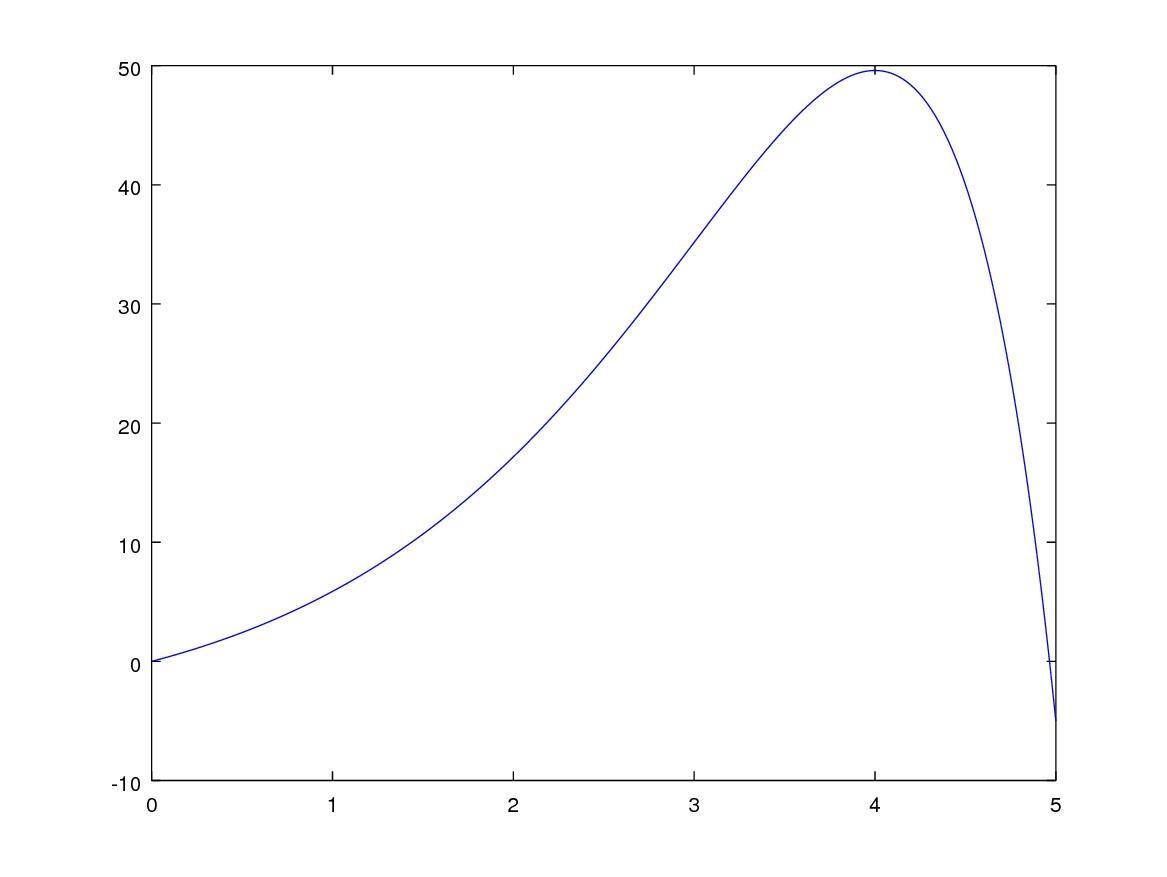
\includegraphics[scale=.5]{../octave/q4fig.jpg}

The interval $I$ after $N$ iterations is $I=2^{-N}$.  Thus if we wanted a interval of $I=10^{-12}$ we would set these as a inequality $10^{-12}\ge 2^{-N}$.  Since $\log$ is monotonic increasing we can take $\log_2$ of both sides $-12\log_2 10\ge -N$.  so we final get $12\log_2 10\ge N$ and the smallest natural with this property is $N=40$.
\newpage
\begin{exercise}{Chapter 4: 2(b)}
\end{exercise}
My newton method
\lstinputlisting{../octave/newton.m}

FINISH LATER NOT DUE TILL NEXT WEEK
\newpage
\begin{exercise}{Chapter 4: 18}
\end{exercise}
let's begin by calculating the derivatives of $f(x)=e^{1-x^2}$.
$$f(x)=e^{1-x^2}$$
$$f'(x)=-2xe^{1-x^2}$$
$$f''(x)=(4x^2-2)e^{1-x^2}$$
$$f'''(x)=(12x-8x^3)e^{1-x^2}$$
Now that we have these it is trivial to crate a Taylor expansion.
\lstinputlisting{../octave/q5.m}
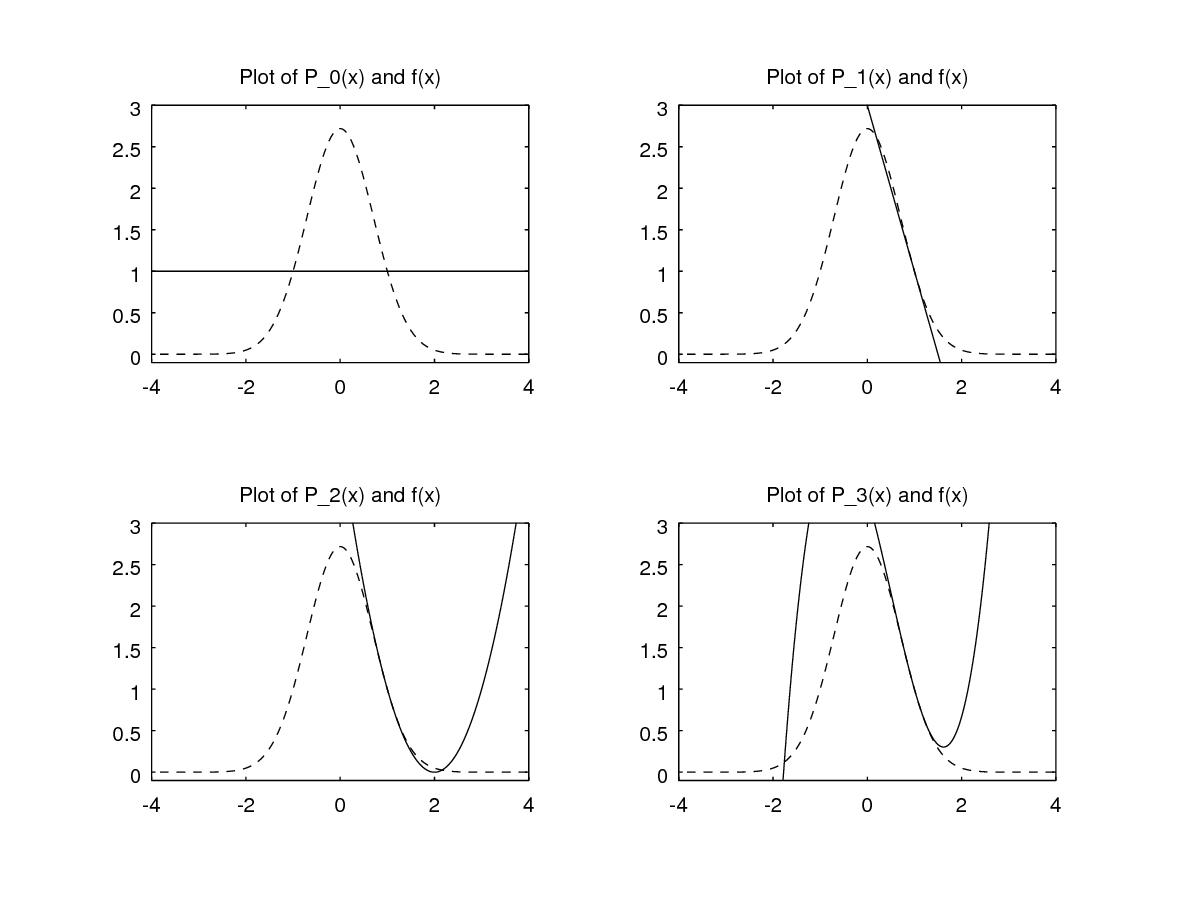
\includegraphics[scale=.9]{../octave/q5fig.jpg}
\end{document}